\begin{frame}{can we get rid of gadgets? (1)}
    \begin{itemize}
    \item Onarlioglu et al, ``G-Free: Defeating Return-Oriented Programming through Gadget-Less Binaries'' (2010)
    \item two parts:
        \begin{itemize}
        \item get rid of unintended jmp, ret instructions
        \item add stack canary-like checks to jmp, ret instructions
        \end{itemize}
    \item hope: no \textit{useful} gadgets b/c of canary-like checks
        \begin{itemize}
        \item all gadgets should be useless without a secret value?
        \item still vulnerable to information leaks
        \end{itemize}
    \item overhead is not low:
        \begin{itemize}
        \item 20--30\% (!) space overhead
        \item 0--6\% time overhead
        \end{itemize}
    \end{itemize}
\end{frame}

\begin{frame}{no unintended jmp/ret (1)}
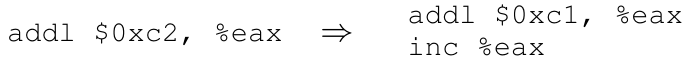
\includegraphics[width=10cm]{../mitigate/gfree1}
\begin{itemize}
\item \texttt{addl \$0xc2, \%eax}: \texttt{05 \myemph<2>{c2 00 00} 00}
\item problem: \texttt{\myemph<2>{c2 00 00}}: variant of ret instruction
\item paper's proposed fix: change the constant
\end{itemize}
\end{frame}

\begin{frame}{no unintended jmp/ret (2)}
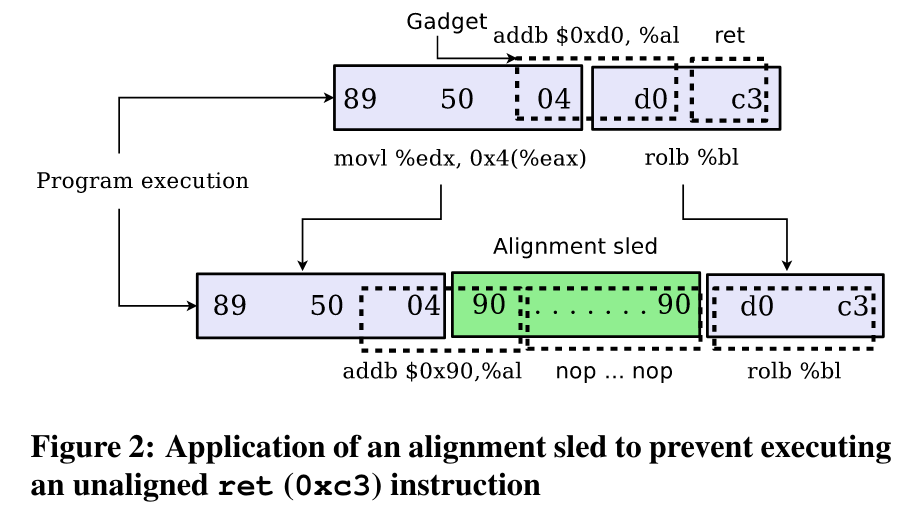
\includegraphics[width=10cm]{../mitigate/gfree2}
\end{frame}
